%
% buchcover.tex -- Cover für das Buch 
%
% (c) 2017 Prof Dr Andreas Müller, Hochschule Rapperswil
%
\documentclass[11pt]{standalone}
\usepackage{tikz}
\usepackage{times}
\usepackage{geometry}
\usepackage[utf8]{inputenc}
\geometry{papersize={405mm,278mm},total={405mm,278mm},top=72.27pt, bottom=0pt, left=72.27pt, right=0pt}

\begin{document}
\begin{tikzpicture}[>=latex, scale=1]
%\clip (0,0) circle (6);

\draw[fill=blue](0,0) rectangle(40.5,27.8);

\begin{scope}
\clip (0,0) rectangle(40.5,27.8);
\node at (26,7.1) [scale=0.125]{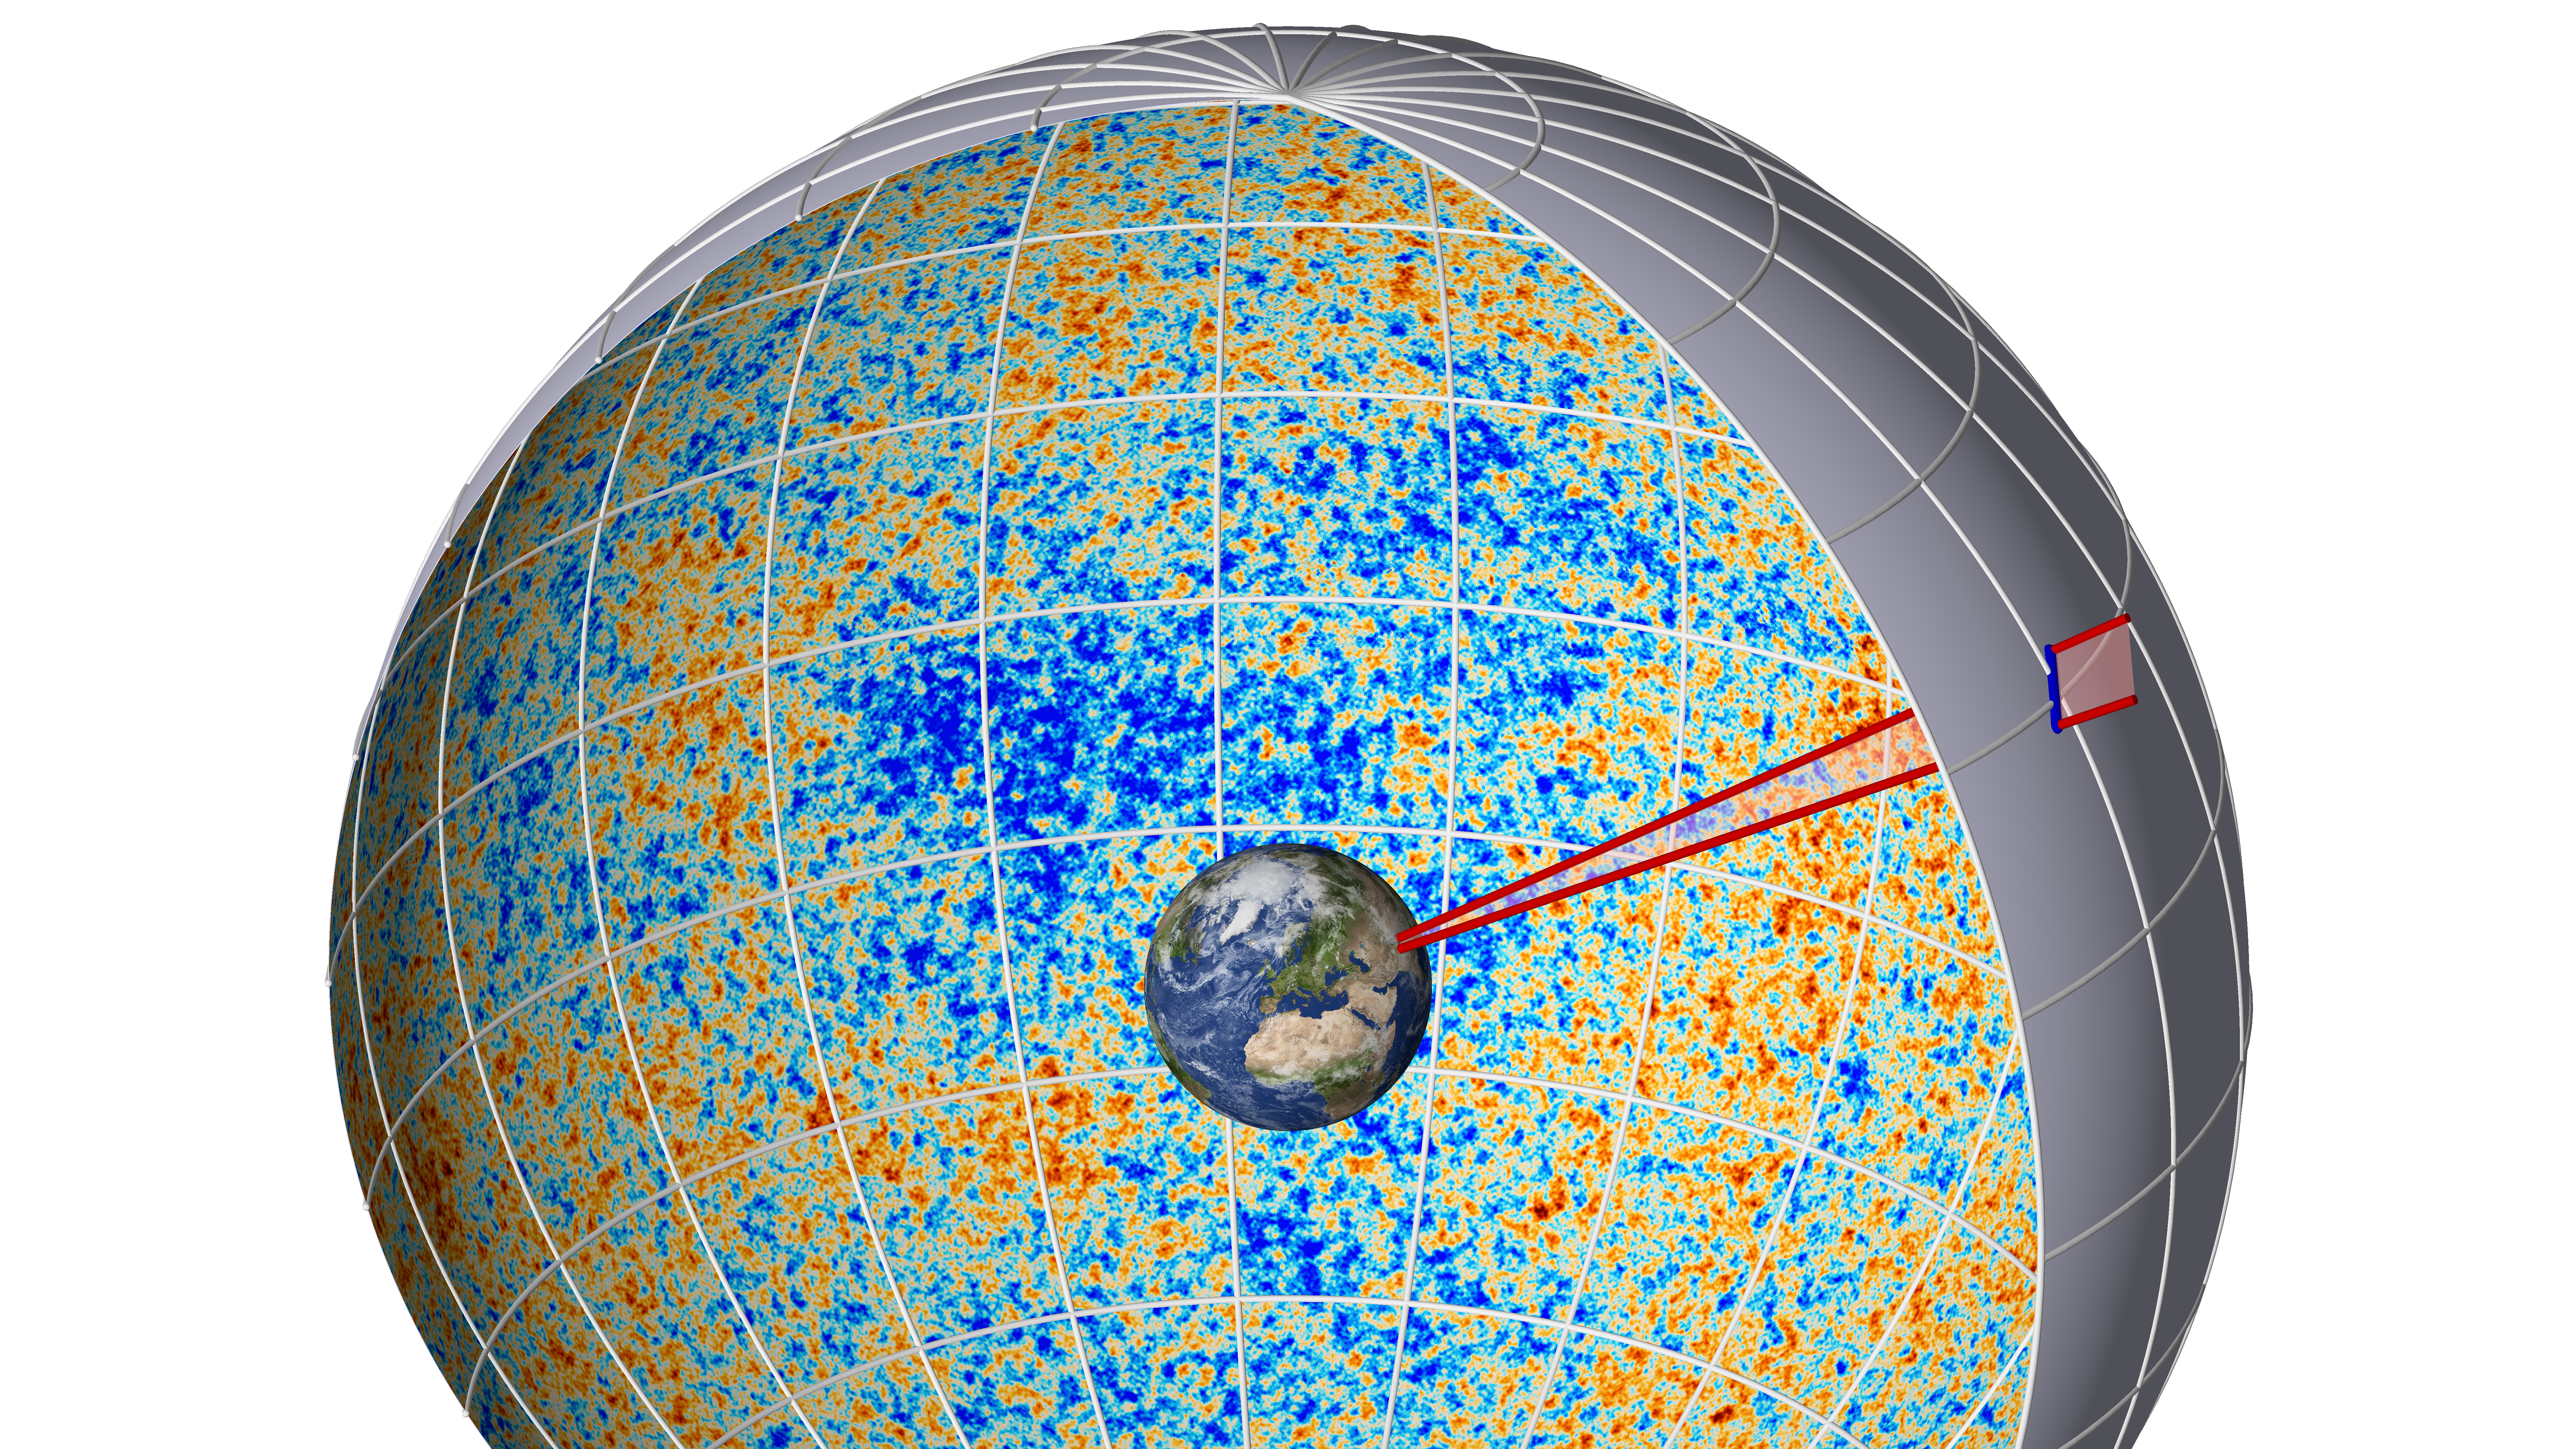
\includegraphics{kugel4-high.png}};
\end{scope}

\node at (29.7,24) [color=white,scale=1] {\hbox to15cm{\hfill%
\sf \fontsize{34}{34}\selectfont Mathematisches Seminar}};
\node at (29.7,20.9) [color=white,scale=1] {\hbox to15cm{\hfill%
\sf \fontsize{60}{70}\selectfont Kosmologie}};

\node at (29.7,18.5) [color=white,scale=1] {\hbox to15cm{\hfill%
\sf \fontsize{13}{5}\selectfont
Jonas Gründler, Sascha Jecklin, Peter Nötzli, Hansruedi Patzen}};
\node at (29.7,17.8) [color=white,scale=1] {\hbox to15cm{\hfill%
\sf \fontsize{13}{5}\selectfont
Nadja Rutz, Fabian Schmid, Kevin Schmidiger, Matthias Schneider}};
\node at (29.7,17.1) [color=white,scale=1] {\hbox to15cm{\hfill%
\sf \fontsize{13}{5}\selectfont
Melina Staub, Pascal Stump, Ambroise Suter, Nico Vinzens}};
 
%\node at (0,3) [color=white] {\sf \LARGE Mathematisches Seminar 2017};

\node at (20.25,20) [color=white,rotate=-90] {\sf\fontsize{35}{0}\selectfont Kosmologie};

\node at (9.95,18) [color=white] {\sf\hsize=13cm
\fontsize{13}{16}\selectfont
\vbox{%
\parindent=0pt
\raggedright
Im Rahmen des Mathematischen Seminars der Hochschule für Technik Rapperswil
wurden im Frühjahrssemester 2017 verschiedene mathematische Methoden
untersucht, die einerseits in der modernen Kosmologie Verwendung finden und
andererseits in der Ingenieurpraxis nützliche Anwendungen haben.
Diese Buch bringt das Skript des Vorlesungsteils mit den von den
Seminarteilnehmern beigetragenen Seminararbeiten zusammen.}};



\draw[white] (0,1.6)--(40.5,1.6);
\draw[white] (0,26.2)--(40.5,26.2);

\draw[white] (1.6,0)--(1.6,27.8);
\draw[white] (18.3,0)--(18.3,27.8);
\draw[white] (19.0,0)--(19.0,27.8);
\draw[white] (21.5,0)--(21.5,27.8);
\draw[white] (22.2,0)--(22.2,27.8);
\draw[white] (38.9,0)--(38.9,27.8);

\end{tikzpicture}
\end{document}
